\documentclass[11pt, oneside]{article}   	% use "amsart" instead of "article" for AMSLaTeX format
\usepackage[margin = 1in]{geometry}                		% See geometry.pdf to learn the layout options. There are lots.
\geometry{letterpaper}                   		% ... or a4paper or a5paper or ... 
%\geometry{landscape}                		% Activate for rotated page geometry
%\usepackage[parfill]{parskip}    		% Activate to begin paragraphs with an empty line rather than an indent
\usepackage{graphicx}				% Use pdf, png, jpg, or eps§ with pdflatex; use eps in DVI mode
								% TeX will automatically convert eps --> pdf in pdflatex		
\usepackage{amssymb}
\usepackage{amsmath}
\usepackage[shortlabels]{enumitem}
\usepackage{float}
\usepackage{tikz-cd}
\usepackage[compat=1.0.0]{tikz-feynman}   %note you need to compile this in LuaLaTeX for diagrams to render correctly
\usepackage{slashed}
\usepackage{simpler-wick}

\usepackage{amsthm}
\theoremstyle{definition}
\newtheorem{definition}{Definition}[section]
\newtheorem{theorem}{Theorem}[section]
\newtheorem{corollary}{Corollary}[theorem]
\newtheorem{lemma}[theorem]{Lemma}

\newcommand{\N}{\mathbb{N}}
\newcommand{\R}{\mathbb{R}}
\newcommand{\Z}{\mathbb{Z}}
\newcommand{\Q}{\mathbb{Q}}

%SetFonts

%SetFonts
\DeclareFontFamily{OMS}{oasy}{\skewchar\font48 }
\DeclareFontShape{OMS}{oasy}{m}{n}{%
         <-5.5> oasy5     <5.5-6.5> oasy6
      <6.5-7.5> oasy7     <7.5-8.5> oasy8
      <8.5-9.5> oasy9     <9.5->  oasy10
      }{}
\DeclareFontShape{OMS}{oasy}{b}{n}{%
       <-6> oabsy5
      <6-8> oabsy7
      <8->  oabsy10
      }{}
\DeclareSymbolFont{oasy}{OMS}{oasy}{m}{n}
\SetSymbolFont{oasy}{bold}{OMS}{oasy}{b}{n}

\DeclareMathSymbol{\smallleftarrow}     {\mathrel}{oasy}{"20}
\DeclareMathSymbol{\smallrightarrow}    {\mathrel}{oasy}{"21}
\DeclareMathSymbol{\smallleftrightarrow}{\mathrel}{oasy}{"24}
%\newcommand{\cev}[1]{\reflectbox{\ensuremath{\vec{\reflectbox{\ensuremath{#1}}}}}}
\newcommand{\vecc}[1]{\overset{\scriptscriptstyle\smallrightarrow}{#1}}
\newcommand{\cev}[1]{\overset{\scriptscriptstyle\smallleftarrow}{#1}}
\newcommand{\cevvec}[1]{\overset{\scriptscriptstyle\smallleftrightarrow}{#1}}

\title{Hadron Structure}
\author{Patrick Oare}
\date{}							% Activate to display a given date or no date

\begin{document}
\maketitle

\section{Deep Inelastic Scattering (DIS)}

This section will begin by studying the Deep Inelastic Scattering (DIS) experiment, which is the process of a high energy 
lepton $\ell$ scattering off of a hadron $h$ via the exchange of a photon, as illustrated in Figure~\ref{fig:dis}. The ``deep 
inelastic" part of the scattering refers to the initial energy of the lepton, which is taken to be very large. DIS is an example 
which will allow us to illustrate most of the interesting features of hadron structure, and we will be able to define many of our 
objects of interest with regards to this type of scattering specifically. 

\begin{figure}[H]
\centering
\feynmandiagram [vertical=a to b] {
  i1 [particle=\(\ell^{-}\)] -- [fermion, edge label'=\(k\)] a -- [fermion, edge label'=\(k'\)] i2 [particle=\(\ell^{-}\)],
  a -- [photon, edge label=\(q\)] b [blob],
  f1 [particle=\(X\)] -- [anti fermion] b -- [anti fermion, edge label'=\(p\)] f2 [particle=\(h\)],
};
\caption{The Deep Inelastic Scattering (DIS) diagram}~
\label{fig:dis}
\end{figure}
%\begin{figure}[H]
%\centering
%    \begin{tikzpicture}
%    \begin{feynman}
%    \vertex (a) {\(e^{-}\)};
%    \vertex [below right=of a] (b);
%    \vertex [above right=of b] (f1) {\(e^-\)};
%    \vertex [below=of b] (c);
%    \vertex [below left=of c] (f2) {\(p^+\)};
%    \vertex [below right=of c] (f3) {\(X\)};
%    \diagram* {
%    (a) -- [fermion] (b) -- [fermion] (f1),
%    (b) -- [boson, edge label'=\(q\)] (c),
%    (c) -- [anti fermion] (f2),
%    (c) -- [fermion] (f3),
%    };
%    \end{feynman}
%    \end{tikzpicture}
%\end{figure}

As the energy of the initial lepton is increased, the transfer momentum $q$ becomes larger and larger until it is able 
to break up the hadron into any particle that is allowed by kinematics and symmetry. As a result, the scattering starts off as 
elastic until it reaches some energy threshold, then becomes highly inelastic as the hadron is smashed into different particles. 
Without any knowledge of the interaction that occurs at the bottom vertex, we can write down a surprising amount of 
information about the scattering process. The amplitude is:
\begin{equation}
	i\mathcal M = -ie\overline u(k')\gamma^\mu u(k) \frac{-ig_{\mu\nu}}{q^2}\hat{\mathcal M^\nu}(q) = 
	-\frac{e}{q^2}\overline u(k')\gamma^\mu u(k)\hat{\mathcal M}_\mu(q)
\end{equation}
where $i\hat{\mathcal M}(q)^\mu$ is the amplitude for the photon interacting with the hadron and breaking it into a final 
state $|X\rangle$, where $|p\rangle$ denotes the hadron state with momentum $p$:
\begin{equation}
i\hat{\mathcal M}^\mu(q) = \int d^4 x\,e^{iqx} \langle X | j_\mu(x) | p\rangle = 
\begin{gathered}
\feynmandiagram [small, vertical=a to b] {
  a [particle=\(\mu\)] -- [photon, edge label=\(q\)] b [blob],
  f1 [particle=\(X\)] -- [anti fermion] b -- [anti fermion] f2 [particle=\(h\)],
};
\end{gathered}~
\label{eq:dis_hadronic_diagram}
\end{equation}
If we want to calculate the unpolarized cross section, then we need the spin averaged matrix element:
\[
	\overline{|\mathcal M|^2} = \frac{1}{2}\sum_{spins, X}|\mathcal M|^2 = \frac{e^2}{2q^4}\left(\sum_{sr}\overline u_r(k')\gamma^\mu 
	u_s(k)\overline u_s(k)\gamma^\nu u_s(k')\right)\left(\sum_\mathrm{spins}\mathcal M_\mu(q)\mathcal M_\nu^*(q)\right)
\]
\begin{equation}
	= \frac{e^2}{2q^4} tr\left[\slashed{k'}\gamma^\mu \slashed{k}\gamma^\nu\right] \left(\sum_\mathrm{spins}\mathcal M_\mu(q)\mathcal M_\nu^*(q)\right)~
	\label{eq:dis_spin_averaged}
\end{equation}
We can integrate this over phase space to get a differential cross section in the lab frame, which we use to define two tensors:
\begin{equation}
	\left(\frac{d\sigma}{d\Omega dE'}\right)_\mathrm{lab} = \frac{\alpha_e^2}{4\pi m_p q^4}L^{\mu\nu} W_{\mu\nu}
\end{equation}

The first tensor $L_{\mu\nu}$ is the \textbf{leptonic tensor} and describes all aspects of the scattering related to the  
initial and final leptons, and how they interact with the photon. Despite not knowing much about the scattering process 
$\gamma^* h\rightarrow X$, we can still explicitly write this tensor down by working through the math starting from 
Equation~\ref{eq:dis_spin_averaged}:
\begin{equation}
	L^{\mu\nu} := \frac{1}{2}tr\left[\slashed{k'}\gamma^\mu\slashed{k}\gamma^\nu\right] = 2(k'^\mu k^\nu + k'^\nu k^\mu - k\cdot k' g^{\mu\nu})
\end{equation}

\subsection{The Hadronic Tensor}

The second tensor $W_{\mu\nu}$ is the \textbf{hadronic tensor}, and describes the physics in the hadronic part of the process, 
namely when the hadron interacts with the mediating photon. Although we do not know many details about the process, we 
can still use general principles of symmetry to make some headway into describing the physics, without explicitly knowing 
information about the final state or the interaction. Explicitly, the hadronic tensor is\footnote{Note that $\mathcal{M}(\gamma^* h\rightarrow X) = \langle X | j_\mu (0) | p\rangle$.}:
\begin{align}
	e^2\epsilon_\mu\epsilon_\nu^* W^{\mu\nu} :=& \left(\frac{1}{2}\right)^2
	\sum_{X, \mathrm{spins}} \int d\Pi_X (2\pi)^6\delta^4\left(\sum p\right)
	|\mathcal M(\gamma^*h\rightarrow X)|^2~
	\label{eq:hadronic_tensor}~
	\\
	& = 2\pi^2 m_{h}|\vec q|\sum_X \sigma(\gamma^*h\rightarrow X)~
	\label{eq:hadronic_tensor_cross}
\end{align}
and depends explicitly on the amplitude for the virtual proton to scatter of the hadron to produce the state $|X\rangle$. 
Notice that the hadronic tensor is proportional to a sum of cross 
sections $\sigma(\gamma^* h\rightarrow X)$-- this fact will be important later. Now, we will use this equation and this 
decomposition to explore the physics of this problem, and will show that we can predict a surprising amount without knowing 
the details of the interaction in Equation~\ref{eq:dis_hadronic_diagram}.

The hadronic tensor can be recast in a more fundamental way for a generic DIS process using the quark electromagnetic 
current 
\begin{equation}
	j^\mu(x) := \sum_q Q_q \overline{q}(x) \gamma^\mu q(x).
\end{equation}
This leads to the following form\footnote{Note that many sources have different normalizations for $W$; generally, you will 
either see this normalization, or this divided by $4\pi$. We will use the conventions from~\cite{quarks_gluons}} for 
$W_{\mu\nu}$:
\begin{align}
	W_{\mu\nu} &= \frac{1}{8\pi} \sum_X\int d\Pi_X \langle ps | j_\mu | X\rangle \langle X | j_\nu | ps \rangle (2\pi)^4 \delta(p + q - 
	p_X)	%\frac{1}{2}\sum_X\int d\Pi_x \int d^4x e^{iqx} \langle p | j_{\mu}(x) | X\rangle \langle X | j_{\nu}(0) | p\rangle 
	\nonumber \\
	&= \frac{1}{4\pi}\int d^4 x\, e^{iqx} \langle ps | [j_\mu(x),\, j_\nu(0)] | ps\rangle
\end{align}
where $s, s'$ are the incoming and outgoing polarizations. For unpolarized scattering, this reduces to:
\begin{equation}
	W_{\mu\nu} = \frac{1}{4\pi}\int d^4 x\, e^{iqx} \langle p | j_\mu(x) j_\nu(0) | p\rangle
\end{equation}

\subsection{Structure Functions and the Compton Tensor}

We can exploit the symmetry of the problem to heavily constrain the form of the hadronic tensor, and 
extract physics from this constrained form. This is the \textbf{method of form factors}. We know the following things about 
$W^{\mu\nu}$ in the case of \textit{unpolarized DIS}:
\begin{enumerate}
	\item It may only depend on the momentum $q^\mu$ and $P^\mu$, since the external momenta in the state $|X\rangle$ 
	are integrated over in the phase space integral. 
	\item It must be symmetric, i.e. $W^{\mu\nu} = W^{\nu\mu}$, because we assume the initial photon is 
	unpolarized\footnote{Bob Jaffe's notes~\cite{jaffe} work with the case that the initial nucleon is polarized. In this case 
	there is an antisymmetric piece to the hadronic tensor, and we will use these notes later to elaborate on this.}. 
	\item It must obey the Ward identity applied to the diagram in Equation~\ref{eq:dis_hadronic_diagram}, so $q_\mu W^{\mu\nu} = 0$. 
\end{enumerate}

Items 1 and 2 on the list say that we can obtain a general form for $W^{\mu\nu}$ by forming all symmetric rank 2 combinations 
of the Lorentz vectors $q^\mu$ and $p^\mu$, as well as the metric $g^{\mu\nu}$, and examining all linear combinations of 
them. This gives 3 parameters we can vary in the linear combination for the general form for $W^{\mu\nu}$. 
However, the Ward identity $q_\mu W^{\mu\nu} = 0$ constrains the form these combinations can take on, and so we actually 
only have 2 coefficients we can vary in the linear combination, which we will call $W_1$ and $W_2$. These coefficients are 
called \textbf{form factors}, and we can explicitly write the most general form of $W^{\mu\nu}$ consistent with our constraints:
\begin{equation}
	W^{\mu\nu}_\mathrm{unpolarized} = \left(-g^{\mu\nu} + \frac{q^\mu q^\nu}{q^2}\right) W_1 + \frac{1}{m_h^2}\left(p^\mu - 
	\frac{p\cdot q}{q^2}q^\mu\right)\left(p^\nu - \frac{p\cdot q}{q^2}q^\nu\right) W_2~
	\label{eq:form_factors}
\end{equation}
There are numerous conventions on the definitions of the structure functions $W_{\mu\nu}$, which typically vary from the 
dimensionality of the quantities. 

If we are studying \textit{polarized DIS}, then a third structure function may be introduced, as the hadronic tensor need not 
be symmetric in this case.
\begin{equation}
	W_\mathrm{pol}^{\mu\nu} = \left(-g^{\mu\nu} + \frac{q^\mu q^\nu}{q^2}\right) W_1 + \frac{1}{m_h^2}\left(p^\mu - 
	\frac{p\cdot q}{q^2}q^\mu\right)\left(p^\nu - \frac{p\cdot q}{q^2}q^\nu\right) W_2 + \frac{i}{2m_h^2} 
	\epsilon^{\mu\nu\alpha\beta}p_\alpha q_\beta W_3
\end{equation}

The form factors $W_1$ and $W_2$ are Lorentz scalars, and therefore must be functions of the Lorentz scalars we can 
generate with our dynamical variables $q^\mu$ and $p^\mu$. The three combinations that we can create are $q^2$, $p^2$, 
and $p\cdot q$. Note that $p^2 = m_h^2$ is not a dynamical variable because we assume the initial photon is on shell, but 
since we do not make this assumption with the photon, $q^2$ is a dynamical variable that our form factors can depend on. 
Thus we can write the form factors as functions of $q^2$ and $p\cdot q$. 

To massage this into a nicer form, let $Q := \sqrt{-q^2}$ be the energy scale of the collision and $\nu := p\cdot q / m_h$. Here 
$\nu$ can also be determined to be the change in energy of the electron due to the scattering, $\nu = E_e - E_e'$. The 
dimensionless ratio:
\begin{equation}
	x := \frac{Q^2}{2 p\cdot q} = \frac{Q^2}{2m_h\nu}
\end{equation}
is called the \textbf{Bjorken variable}, and is an important variable in describing hadron structure. Physically, you can think 
of $x$ as a momentum fraction the photon interacts with in the infinite momentum frame. So, we will consider our form factors 
as functions of $x$ and $Q$:
\begin{equation}
	W_i = W_i(x, Q)
\end{equation}
Note these can equivalently be considered as functions of $(\nu, Q^2)$. 

From the form factors, it is conventional to define \textbf{structure functions} $F_i$ which are proportional to the $W_i$:
\begin{align}
	F_1 := W_1 && F_2 := \frac{\nu}{m_h} W_2 && F_3 := \frac{\nu}{m_h} W_3
\end{align}
The structure functions will sometimes have an additional index $a$ as $F_i^a$, where $a$ denotes the process we are 
discussing, $a = (\ell, h)$ with $\ell \in \{e, \mu, \nu, \overline{\nu}\}$. Each process will generally have a different structure 
function. The \textbf{longitudinal structure function} is also typically defined:
\begin{equation}
	F_L(x, Q^2) := F_2(x, Q^2) - 2x F_1(x, Q^2)
\end{equation}
Written in terms of the structure functions, $W^{\mu\nu}$ becomes:
\begin{equation}
	W^{\mu\nu} = \left(-g^{\mu\nu} + \frac{q^\mu q^\nu}{q^2}\right) F_1 + \frac{1}{m_h\nu}\left(p^\mu - 
	\frac{p\cdot q}{q^2}q^\mu\right)\left(p^\nu - \frac{p\cdot q}{q^2}q^\nu\right) F_2 + \frac{i}{2m_h\nu} 
	\epsilon^{\mu\nu\alpha\beta}p_\alpha q_\beta F_3
\end{equation}

Using the general form Equation~\ref{eq:form_factors} of the hadronic tensor, we can plug this into our cross section to 
express it explicitly in terms of $W_1$ and $W_2$:
\begin{equation}
	\left(\frac{d\sigma}{d\Omega dE'}\right)_{lab} = \frac{\alpha_e^2}{4 m_h E^2\sin^4(\theta / 2)}\left(W_2(x, Q)
	\cos^2\frac{\theta}{2} + 2W_1(x, Q)\sin^2\frac{\theta}{2}\right)~
	\label{eq:sigma_ff}
\end{equation}
This should be pretty remarkable: without knowing anything about the final state $|X\rangle$ or really any details of the 
hadronic process described by the diagram of Equation~\ref{eq:dis_hadronic_diagram}, we have expanded an observable in 
terms of the two form factors $W_1$ and $W_2$. This means that the form factors can be experimentally measured, and then 
we can use those measurements to make other predictions about the process. 

The typical way to compute the hadronic tensor is to relate it to a time ordered 
quantity called the \textbf{Compton tensor}:
\begin{equation}
	T_{\mu\nu} := i\int d^4 x\, e^{iqx}\langle p | T\{j_{\mu}(x)\, j_{\nu}(0)\} | p\rangle
\end{equation}
Because $T_{\mu\nu}$ is a time ordered correlator, \textit{it can be calculated on the lattice or in perturbation theory}. 

$T_{\mu\nu}$ is important to the study of DIS because it can also be expanded with form factors:
\begin{equation}
	T^{\mu\nu} = \left(-g^{\mu\nu} + \frac{q^\mu q^\nu}{q^2}\right) T_1 + \frac{1}{m_h\nu}\left(p^\mu - 
	\frac{p\cdot q}{q^2}q^\mu\right)\left(p^\nu - \frac{p\cdot q}{q^2}q^\nu\right) T_2 + \frac{i}{2m_h\nu} 
	\epsilon^{\mu\nu\alpha\beta}p_\alpha q_\beta T_3
\end{equation}
with $T_3$ again vanishing for unpolarized scattering. The structure functions can be related to the structure functions of the hadronic tensor via the optical theorem:
\begin{equation}
	F_i^a = \frac{1}{2\pi} T_i^a
\end{equation}
for $i = 1, 2, 3$. 

\subsection{The Parton Model}

A \textbf{parton} is a point-like particle which has no composite substructure-- examples of partons are the electron, neutrino, 
and quarks. When nuclear structure was being studied, the proton was originally believed to be a parton as well until 
experiments like DIS showed that it instead has a substructure of quarks and gluons. 

Feynman coined the \textbf{parton model} of the proton, in which he assumed the proton was made up of constituent 
partons that interact weakly and are almost free particles. Suppose that we assume the proton is made up of partons of mass 
$\{m_i\}_{i}$. In DIS, we can assume the photon interacts with a single parton, say parton $j$. Then we can describe this 
process with the diagram in Figure~\ref{fig:dis} where we replace the proton line with a parton line with incoming momentum 
$p_j$ and external momentum $p_j'$. Momentum conservation gives us $p_j + q = p_j'$, and squaring both sides we get:
\begin{equation}
	\frac{Q^2}{2p_j\cdot q} = 1
\end{equation}
Since the parton is a constituent of the proton with momentum $P$, assume that it has a fraction $\xi$ of the proton's 
momentum $P$, i.e. $p_j = \xi P$. Then using the equation above, we find the Bjorken variable is:
\begin{equation}
	x = \frac{Q^2}{2P\cdot q} = \xi \frac{Q^2}{2p_j\cdot q} = \xi
\end{equation}
so with these assumptions, the Bjorken $x$ is exactly the momentum fraction of the parton which is involved in the scattering 
process. 

Note that in the physical world described fully by QCD, the Bjorken variable is not the momentum fraction of the 
parton. This will be approximately true, \textbf{but in general $x$ and $\xi$ are different, although they are related; they are 
only equal in the infinite momentum (lightcone) frame}. Thinking of the physical interpretation of $x$ as the momentum fraction 
is helpful, but not exactly accurate. If we look at the previous bit of work we did which showed $x = \xi$, there was an additional 
assumption we made that we are working in the lightcone frame. If we don't work in the lightcone frame, we \textit{cannot assume 
that $p_i$ and $P$ are linearly dependent, i.e. we cannot generally write $p_i^\mu = \xi P^\mu$ unless we are in the DIS limit}. 
For example, in the rest frame of the proton, if the parton has nonzero three momentum $\vec p_i\neq 0$, then we can't write 
$p_i^\mu = \xi P^\mu$. Essentially by taking the lightcone limit, we're removing the different mass scales of the parton and the proton 
from the problem, and their lightcone components can then be taken to be linearly dependent. 

In the actual proton, partons are not free but interact. Assuming they interact via the electromagnetic force, we can 
examine the process $e^-q\rightarrow e^-q$ through a photon exchange, where $q$ is the parton. When we studied IR 
divergences, we calculated this for the $e^-e^+\rightarrow\mu^-\mu^+$ scattering, and found that the form factor $F_1(q^2)$ 
ran as $F_1(q^2)\propto log(Q^2)$ and $log^2(Q^2)$ when the initial momentum was fixed (i.e. when we vary $x$). This weak 
running of the form factors as we vary $Q$ at fixed $x$ is called \textbf{Bjorken scaling} and applies in the parton model as 
well: when we work at fixed $x$: the form factors stay relatively constant as we vary the energy scale of the collision. 
Specifically, Bjorken scaling states that in the \textbf{DIS limit where $Q^2\rightarrow\infty$, the structure functions are 
independent of $Q^2$ and only depend on $x$}.

Another key ingredient of the parton model is an object known as a \textbf{Parton Distribution Function (PDF)}. PDFs are 
functions $f_i(\xi)d\xi$ which give the probability density for scattering off of parton $i$ having momentum fraction $\xi$. Since 
the Bjorken variable has an interpretation as the momentum fraction of the proton which is contained by the parton, we will 
write out PDFs as $f_i(x)dx$. The parton model assumes that we can factorize the DIS cross section into partonic ones:
\begin{equation}
	\sigma(e^- P^+\rightarrow e^- X) = \sum_i\int_0^1dx f_i(x)\hat{\sigma}(e^- p_i\rightarrow e^- X)~
	\label{eq:sigma_pdf}
\end{equation}
Here the sum runs over all partons $p_i$ contained in the proton, and $\hat\sigma$ is the cross section for the partonic 
process. 

Now, we assume that the partons only interact with the proton through QED and have charges $Q_i$ ($Q_i$ is the electric 
charge of different types of quarks). This allows us to use the Rosenbluth formula for spin 1/2 QED scattering with form factors 
$F_1\equiv 1$ and $F_2\equiv 0$. Plugging these into Equation~\ref{eq:sigma_pdf} and turning it into a differential cross 
section, we can compare it to Equation~\ref{eq:sigma_ff} to read off the structure functions $F_1$ and $F_2$:
\begin{align}
	F_1(x, Q) = \frac{1}{2}\sum_i Q_i^2 f_i(x) && F_2(x, Q) = x\sum_i Q_i^2 f_i(x)~
	\label{eq:ff_decomp}
\end{align}
The relation between $F_1$ and $F_2$ is called the \textbf{Callan-Gross relation}, and was used as experimental evidence for 
the parton model. It is a direct consequence of the fact that quarks have spin 1/2. The relation is:
\begin{equation}
	F_2(x, Q) = 2x F_1(x, Q)
\end{equation}
Note that \textit{this equation, as well as most others in this section, only applies in the deep inelastic (infinite momentum) limit where 
$Q^2\rightarrow\infty$}. In the general case, the relationship between $F_1$ and $F_2$ is typically expressed in terms of the ratio of 
longitudinal to transverse cross sections:
\begin{equation}
	R := \frac{\sigma_L}{\sigma_T} = \frac{F_2}{2x F_1}\left(1 + 4 \frac{m_h^2x^2}{Q^2}\right) - 1~
	\label{eq:R_F2}
\end{equation}
This ratio $R$ is shown to be independent of the target in experiments, and relatively small.\footnote{``Small" here means that for $x \geq
0.1$, measured values of $R$ tend to be $\leq 0.1$~\cite{nuclear_emc}.} 

Equation~\ref{eq:ff_decomp} allow us to write out the proton form factors in terms of PDFs (note here we adopt the notation that the pdf 
$q(x) := f_q(x)$, so for example we use $u(x)$ to denote $f_u(x)$). We can see that the proton has $F_2$ form factor:
\begin{equation}
	F_2(x, Q) = x\left(\frac{4}{9} u + \frac{4}{9}\bar u + \frac{1}{9} d + \frac{1}{9}\bar d+ \frac{1}{9} s + \frac{1}{9}\bar s + ...\right)
\end{equation}
This can then be used to determine the form factors of the neutron, using isospin symmetry $u\leftrightarrow d$. 

PDFs must satisfy certain constraints to be valid probability distributions: namely, they must satisfy certain \textbf{sum rules} 
related to particle number conservation. As an example of this, consider the up quarks in the proton. While at any given time 
there are 2 valence quarks, we can also have $q\overline q$ production to create sea quarks. Since the total number of up 
quarks is conserved ($N_u + N_{\bar u} = 2$) we must have:
\begin{equation}
	\int_0^1dx \left(f_{u}(x) - f_{\bar u}(x)\right) = 2
\end{equation}
because for a single quark PDF, the total integral $\int_0^1dx\,q(x) = N_q$. Similar rules hold in the proton for down ($N_d = 
1$) and other flavor ($N_f = 0$ for $f = s, c, b, t$) quarks. In general, a sum rule will apply anytime there is a conserved particle 
number. The proton is a bound state with specific quantum numbers for its number of (each flavor of) quarks, which implies the 
sum rules for the quark PDFs. Since specifying a bound hadron or meson state also specifies its quantum numbers, this 
means that \textit{each bound QCD state will come with its own set of sum rules} to reflect its general make-up. Note because 
gluon number is not conserved, there is \textit{no general sum rule for the gluon PDFs in a QCD bound state}. There is also an 
additional sum rule for momentum conservation:
\begin{equation}
	\sum_i \int_0^1 dx\, x f_i(x) = 1
\end{equation}
where $f_i$ ranges over all PDFs in the nucleon, including the gluon. 

Many sum rules allow us to probe the structure of the nucleon directly through experiments by relating the PDFs in the nucleon to its 
structure functions. Sum rules allow us to quantify how much nucleon structure deviates from what we expect by looking at integrals of 
structure functions. For example, consider the \textbf{Adler sum rule} in the proton. Since there 
is always one extra valence up quark than down quark in the proton, the Adler sum rule allows us to experimentally verify the fact that:
\begin{equation}
	\int_0^1dx\left[(u - \overline u) - (d - \overline d)\right] = 1
\end{equation}
Expanding out the PDFs in terms of structure functions, one obtains the prediction:
\begin{equation}
	S_\mathrm{A} = \int_0^1dx\left[ F_1^{\overline \nu, p}(x, Q^2) - F_1^{\nu, p}(x, Q^2)\right] = 1
\end{equation}
where the structure functions $F_1^{\nu, p}$ and $F_1^{\overline\nu, p}$ are determined through neutrino and anti-neutrino DIS. These 
integrated structure functions can be experimentally determined to show that the physics in the proton behaves as we would expect for 
this prediction.

For a less trivial example, consider the \textbf{Gottfried sum rule}. Here, we can relate the difference in $F_2$ structure functions between 
the proton and neutron to their PDF decomposition:
\begin{equation}
	F_{2, p} - F_{2, n} = \frac{x}{3}\left[(u + \overline u) - (d + \overline d)\right]
\end{equation}
We can massage this into a new sum rule:
\begin{align}
	S_\mathrm{G} &= \int_0^1\frac{dx}{x}(F_{2, p} - F_{2, n}) = \frac{1}{3} S_\mathrm{A} - \frac{2}{3} \int dx\, (\overline d - \overline u) \\
	&= \frac{1}{3} - \frac{2}{3}\int dx\,(\overline d - \overline u)
\end{align}
Perturbative QCD predicts that $\overline u$ and $\overline d$ in the proton should be the same (or very close to identical), since their 
masses are almost degenerate and a gluon should decay into either a $u\overline u$ pair with exactly the same frequency as a $d\overline d$ 
pair. In this case, we would predict $S_\mathrm{G} = \frac{1}{3}$. However, this quantity has been experimentally verified and it is \textit{not 
equal to $\frac{1}{3}$}, which explicitly shows a deviation from perturbative QCD, and shows that we must embrace full, non-perturbative 
QCD to study the full structure of the nucleon. The fact that $S_\mathrm{G}\neq\frac{1}{3}$ is thought to result from pions (Goldstone 
modes) in chiral symmetry breaking, which we will discuss at a future point.

\subsection{OPE in DIS}

The OPE is used in DIS to expand out the time ordered product $\langle 0 | T\{j_\mu(x) j_\nu(0)\} | 0 \rangle$ into a sum of 
local operators with unspecified Wilson coefficients. Recall that the \textbf{twist} of an operator 
$\mathcal{O}_{\mu_1 ... \mu_s}$ with mass dimension $d := [\mathcal{O}_{\mu_1 ... \mu_s}]$ is:
\begin{equation}
	\tau := d - s
\end{equation}
Twist is important to consider in the OPE because \textbf{an operator's contribution to the OPE decreases as its twist 
increases}; the operators with lowest twist, starting at twist 2, are the most relevant to the computation, and the higher-twist 
operators are subleading in the expansion. This is because when everything is worked out, an operator with twist $\tau = 2 + 
2n$ will have Wilson coefficients scaling as $(m_h^2 / Q^2)^n$, and $Q^2\rightarrow\infty$ in the DIS limit. 

The basis of twist-2 operators we can form from quark and gluon fields contains 3 types of operators. The first operator does 
not transform as a singlet under $SU(3)$:
\begin{equation}
	\mathcal{O}_{NS, \pm}^{\mu_1 ... \mu_n a} := \overline q(x) T^a \gamma^{\{\mu_1}D^{\mu_2} ... D^{\mu_n\}} q(x)
\end{equation}
The other two operators are $SU(3)$ singlets:
\begin{align}
	\mathcal{O}_{q}^{\mu_1 ... \mu_n} &:= \overline q(x) \gamma^{\{\mu_1} D^{\mu_2} ... D^{\mu_n\}}q(x) \\
	\mathcal{O}_{g}^{\mu_1 ... \mu_n} &:= F^{\{\mu_1\nu} i D^{\mu_2} ... i D^{\mu_{n - 1}} F^{\mu_n\nu\}}
\end{align}
where $\{\}$ denotes symmetrization and trace subtraction. Note they both are pieces in the QCD EMT. A computation can be 
done to evaluate the $SU(3)$ singlet part of $T_{\mu\nu}$ with the OPE by expanding $T\{j_\mu(x) j_\nu(0)\}$ as a linear combination of the 
operators $\mathcal{O}_q$ and $\mathcal{O}_g$, and we find that the quark operator contributes as:
\begin{equation}
	T_{\mu\nu} = \sum_q Q_q^2\left[\left(-g^{\mu\nu} + \frac{q^\mu q^\nu}{q^2}\right)\sum_{n = 2, 4, ...} 
	\frac{M_q^n}{x^n} + \frac{4 x^2}{Q^2}\left(p^\mu - \frac{p\cdot q}{q^2}q^\mu\right)\left(p^\nu - 
	\frac{p\cdot q}{q^2}q^\nu\right)\sum_{n = 2, 4, ...} \frac{M_q^n}{x^n}\right]
\end{equation}
where here $M_q^n$ are the \textbf{Mellin moments} for the quark $q$:
\begin{equation}
	M_q^n := \int_0^1 dx\, x^{n - 1} f_q(x)
\end{equation}
which appear as coefficients in the matrix elements of the OPE operators, $\langle p | \mathcal{O}_q^{\mu_1 ... \mu_n} 
| p\rangle = M_q^n p^{\{\mu_1} ... p^{\mu_n\}}$. Using this, we can read off the structure functions for the Compton 
tensor:
\begin{align}
	T_1 = \sum_q Q_q^2\sum_{n = 2, 4, ...}\frac{M_q^n}{x^n} && T_2 = 2x\sum_q Q_q^2\sum_{n = 2, 4, ...}
	\frac{M_q^n}{x^n}
\end{align}
This makes it clear that the Mellin moments define the PDF, since we have $F_2 = \frac{1}{2\pi} T_2 = x \sum Q_i^2 f_i$:
\begin{equation}
	f_q(x) = \frac{1}{\pi} \sum_{n = 2, 4, ...} x^{-n} \mathrm{Im}M_q^n
\end{equation}

The evolution of Mellin moments can be determined from perturbative QCD with the DGLAP equations; we will defer discussion of 
the evolution equations until our discussion of DGLAP in Section~\ref{ch:dglap}.

\subsection{The EMC Effect}

The \textbf{EMC effect} was the one of the first pieces of experimental evidence that nucleons as a composite object behave differently than 
the sum of their parts. The effect was published in 1983 by the European Muon Collaboration (EMC)~\cite{emc_effect} and shows a difference
in the structure function $F_2$ per nucleon between iron and deuterium. It quantifies the difference between the naive picture of the nucleus 
as a composite particle made from packing protons and neutrons together, and the picture of the nucleon in full QCD, where the nucleus is a 
bag of quarks and gluons which are not bound in individual protons and neutrons. The former model is an effective theory of QCD, and the 
deviation in the EMC effect ratio from unity quantifies the failure of this EFT to predict the full theory of QCD.

Namely, the EMC computed the ratio $F_2^N(x; \mathrm{Fe}) / F_2^N(x, \mathrm{D})$, where $F_2^N$ is the $F_2$ value per nucleon, Fe is 
iron, and De is deuterium. If the nucleon was simply composed of composite protons and neutrons, then the physics of $^{56}\mathrm{Fe}$ 
and $^2\mathrm{He}$ would be identical, up to scaling from the amount of nucleons. However, the EMC found the result in 
Figure~\ref{fig:emc_effect}. 
\begin{figure}[H]
	\centering
	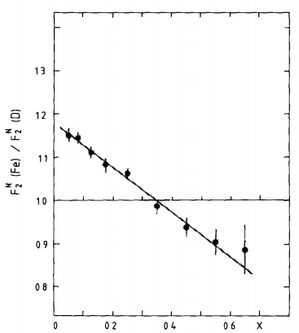
\includegraphics[width = .5\textwidth]{emc_effect}
	\caption{Ratio of the structure function per nucleon in iron vs. deuterium~\cite{emc_effect}.}~
	\label{fig:emc_effect}
\end{figure}

The EMC effect refers to the region of this graph with $x\in [0.3, 0.6]$. Using the naive EFT of the nucleus, one would expect this structure 
function ratio to equal unity, since it is normalized per number of nucleons. This deviation has been reproduced in numerous different targets 
and is a now a well accepted discrepancy between experiment (predicted by full QCD, which can be done on the lattice) and the nucleus 
EFT.

In this EFT, the only existing explanation for a deviation in $F_2$ per nucleon for different nuclei would be from \textbf{Fermi motion}, which 
is the quantum mechanical motion of nuclei inside the nucleon. This is due to nuclei being confined in a finite amount of space and subject to 
the uncertainty principle, and so at any given time we cannot know the true momentum of a nucleon. The EMC considered this before 
publishing the paper detailing the EMC effect, and Fermi motion cannot account for most of the data.

Many models have been made to incorporate this effect into our current effective theories which nucleons (mostly) follow, and we will 
elaborate on a few. The most popular model of the EMC effect is called \textbf{short range correlations}. 

Lattice QCD calculations allow us to calculate QCD predictions from first principles. As a result, although we cannot verify any of these 
models directly, we can exclude certain models if their predictions do not match lattice calculations. 

\newpage
\section{Other processes and form factors}

Deep inelastic scattering is the most widely studied process in QCD, but there are many more interactions one can consider. 
Much of the theory in these processes is very similar to DIS, but we will specifically be interested in laying out the different structures 
and form factors that can arise in these alternate settings. 

Form factors up to now may seem reasonably abstract, since their definition is as expansion coefficients for a combination of matrix 
elements constrained from symmetry. \textit{The general interpretation of form factors is that upon Fourier transforming them, one gets a 
density in position space}. The type of density and information it contains is specific to the form factor of interest; we will see some examples 
of this in the next section.

\subsection{Electron-nucleon scattering}

Electron-nucleon scattering is exactly what it sounds like: an electron scattering elastically off a nucleon. Experimentally, this process is 
the same as DIS except at a moderate $Q^2$ value, and we do not take the DIS limit $Q^2\rightarrow\infty$. As such, the nucleon doesn't 
shatter into little pieces and stays intact throughout the whole process. The hadronic tensor is much simpler to write down than DIS because 
the nucleon is kept intact:
\begin{equation}
	W_{\mu\nu}^{e^-p^+} = \langle P | j_\nu | P'\rangle \langle P' | j_\mu | P\rangle
\end{equation}
where $j_\mu$ is the electromagnetic current and $|P\rangle$, $|P'\rangle$ are the initial and final nucleon states with momentum $P$ and 
$P'$, respectively. In this case, we don't expand the hadronic tensor fully in terms of form factors, but rather the current matrix element. 

Expanding the matrix element yields two form factors (much like in the case of studying the electron's anomalous magnetic moment):
\begin{equation}
	\langle P' | j_\mu(q) | P\rangle = \overline{u}(P')\left(\gamma^\mu F_1(Q^2) + i\sigma_{\mu\nu} \frac{q^\nu}{2m_n} F_2(Q^2)\right) u(P)
\end{equation}
Here $F_1(q^2)$ is called the \textbf{Dirac form factor} and $F_2(q^2)$ is called the \textbf{Pauli form factor}. These two form factors 
are subject to the \textbf{dimensional scaling rule}, which comes from factorization and evaluation of the perturbative pieces making up each 
form factor. The scaling rule says that asymptotically as $Q^2\rightarrow\infty$, the general scaling behavior of these form factors is:
\begin{align}
	F_1(Q^2)\xrightarrow{Q^2\rightarrow\infty} \frac{C_1}{Q^4} && F_2(Q^2)\xrightarrow{Q^2\rightarrow\infty} \frac{C_2}{Q^6}
\end{align}
From $F_1$ and $F_2$, it is conventional to define the \textbf{Sachs electric and magnetic form factors}:
\begin{align}
	G_\mathrm{E}(Q^2) &:= F_1(Q^2) - \frac{Q^2}{4 m_n^2} F_2(Q^2) \\
	G_\mathrm{M}(Q^2) &:= F_1(Q^2) + F_2(Q^2)
\end{align}
The Sachs form factors are subject to the following normalizations at $Q^2 = 0$, which explains the reason for the nomenclature:
\begin{align}
	G_\mathrm{E}^{p^+}(0) = 1 && G_{\mathrm M}^{p^+}(0) = \mu_p \\
	G_\mathrm{E}^{n^0}(0) = 0 && G_{\mathrm M}^{n^0}(0) = \mu_n
\end{align}
where $\mu_p$ and $\mu_n$ are the proton and neutron magnetic moments. As $Q^2$ varies, the Sachs electric form factor 
$G_\mathrm{E}^{n^0}(Q^2)$ of the neutron does not stay zero, but rather has has some dependence on $Q^2$. This is indication that the 
\textit{neutron has electric structure}; despite the total charge being 0, the neutron has a charge radius and its electric charge density forms 
a nonzero cloud around the particle. Other combinations of these form factors that are also 
considered are \textbf{isoscalar} and \textbf{isovector} combinations of $F_1$ and $F_2$ for the proton and the neutron:
\begin{align}
	F_{1, 2}^\mathrm{S} = \frac{1}{2}\left(F_{1, 2}^{p^+} + F_{1, 2}^{n^0}\right) && F_{1, 2}^\mathrm{V} = \frac{1}{2}\left(F_{1, 2}^{p^+} - 
	F_{1, 2}^{n^0}\right)
\end{align}
Generally, anytime we denote a form factor with a $S$ or a $V$, we will mean the same isoscalar or isovector combination that we do here. 

All of this is typically considered in the rest frame of the nucleon, but other frame choices often simplify matters. The \textbf{Breit frame} is 
the center of momentum frame, where the incoming electron has three momentum $\vec p = \frac{1}{2}\vec q$ and the proton has three 
momentum $\vec P = -\frac{1}{2}\vec q$. The scattering is elastic, so the outgoing electron has $\vec p' = -\frac{1}{2}\vec q$, and the outgoing 
proton has $\vec P' = \frac{1}{2}\vec q$. In the Breit frame, the current matrix elements are simple and give the interpretation of the 
Sachs form factors:
\begin{align}
	\langle N_{s'}(\vec q / 2) | j^0(0) | N_s(-\vec q / 2)\rangle &= 2 m_n G_\mathrm{E}(\vec q^{\;2})\delta_{s, s'} \\
	\langle N_{s'}(\vec q / 2) |\, \vec j (0)\,| N_s(-\vec q / 2)\rangle &= G_\mathrm{M}(\vec q^{\;2})\chi_{s'}^\dagger i(\vec\sigma\times\vec q) 
	\chi_s 
\end{align}
We see that we can interpret $G_\mathrm{E}(q^2)$ as an electric charge density and $G_\mathrm{M}(q^2)$ as a magnetization density.
Formally, the charge density is the Fourier transform of $G_\mathrm{E}$:
\begin{equation}
	\rho(\vec r) = \int\frac{d^3\vec q}{(2\pi)^3} e^{-i\vec q\cdot\vec r} \frac{m_n}{E(\vec q\,)} G_\mathrm{E}(\vec q^{\,2})
\end{equation}
The  \textbf{charge radius of the nucleon} is defined in terms of $G_\mathrm{E}$ as:
\begin{equation}
	\langle r^2\rangle_\mathrm{E} := -6 \frac{1}{G_\mathrm{E}(0)}\frac{d G_\mathrm{E}(Q^2)}{dQ^2}\bigg|_{Q^2 = 0}~
	\label{eq:charge_radius}
\end{equation}
In the Breit frame for the limit of $m_n\rightarrow\infty$, the expression for $\langle r^2\rangle$ reproduces its 
value from classical electrostatics with charge density $\rho(r)$ as\footnote{Classically, we have $\langle r^2\rangle = \int d^3\vec r \rho(\vec 
r\,) r^2 = 4\pi \int dr \, r^2 \rho(\vec r) r^2$.}:
\begin{equation}
	\langle r^2\rangle_\mathrm{E}^\mathrm{Breit} = 4\pi\int_0^\infty dr\, r^4\rho(r)
\end{equation}
which further reinforces the interpretation of the F.T. of $G_\mathrm{E}(Q^2)$ as the charge density. For the proton, the value of 
$\langle r^2_\mathrm{E}\rangle$ and $\langle r^2\rangle_\mathrm{M}$\footnote{$\langle r^2\rangle_\mathrm{M}$ is defined analogously to 
Eq.~(\ref{eq:charge_radius}).} is a little under $1\textnormal{ fm}$.


\subsection{Neutron $\beta$-decay}

Studying the $\beta$ decay of the neutron allows us to study the weak decays allowed in the Standard Model which are facilitated by 
neutral currents. Such currents are typically called \textbf{Flavor Changing Neutral Currents} (FCNCs), as they are neutral currents 
which change the flavor of quarks. 

The lifetime of a free neutron outside a nucleus to decay to a proton through $\beta$-decay is a mere 15 minutes. 

\subsection{Drell-Yan}


\newpage
\section{Parton Distribution Functions (PDFs)}

\subsection{Lightcone coordinates and PDFs}

This section will pull from~\cite{pdfs} and Schwartz and aim discuss PDFs in some generality. A lightcone momentum (boosted 
in the $z$ direction) is a generalization of a massless momentum. For a massive particle with momentum $p_\mu$, the 
lightcone limit is where $|\vec p|^2\rightarrow\infty$, as in this case $p^0\approx |\vec p|$. Vectors on the lightcone are expanded 
in the basis:
\begin{align}
	n_\mu := \begin{pmatrix} 1 \\ 0 \\ 0 \\ 1 \end{pmatrix} && \overline{n}_\mu := \begin{pmatrix} 1 \\ 0 \\ 0 \\ -1 \end{pmatrix}
\end{align}
These vectors are defined to satisfy:
\begin{align}
	n^2 = 0 && n\cdot \overline{n} = 2 && \overline{n}^2 = 0
\end{align}
with projectors $\slashed{n}$ and $\slashed{\overline{n}}$ projecting a Dirac spinor $\psi$ onto its positive and negative 
lightcone components. A general four vector $p_\mu$ can be decomposed as:
\begin{equation}
	p^\mu = \frac{1}{2}(\overline n\cdot p) n^\mu + \frac{1}{2} (n\cdot p)\overline{n}^\mu + p_\perp^\mu
\end{equation}
where $p_\perp^\mu$ is a transverse momentum to $n^\mu$ and $\overline{n}^\mu$ with only $x$ and $y$ components. 

For the definition of a PDF on the lightcone, consider a a parton $f$ in a hadron $H$. Take the hadron to be moving in the 
$\hat{n}_\mu$ direction with momentum is $P_\mu = P\overline{n}_\mu$, so its three momentum is oriented opposite the 
positive direction specified by $n_\mu$. Let $x\in [0, 1]$ be the momentum fraction of the parton in $H$, i.e. the partonic 
momentum $p$ is:
\begin{equation}
	n\cdot p = x(n\cdot P)
\end{equation}
Notice that $n\cdot p$ is the component of $p$ along $\overline{n}_\mu$, and that we only enforce the momentum fraction 
along the $\hat{n}_\mu$ direction, so that we can allow for transverse perturbations. In general, the partonic momentum 
is $p^\mu = (n\cdot p)\overline{n}^\mu + p_\perp^\mu$, where $p_\perp^\mu$ a small transverse momentum with $p_\perp^\mu\approx 
0$. Furthermore, $x$ will coincide with the Bjorken variable. 

Because $f(x)$ is the probability of finding such a parton, we can explicitly write down a formula for $f$ as:
\begin{equation}
	f(x) = \sum_X\int d\Pi_X |\langle X | \psi_f | P\rangle |^2 \delta\left(x(n\cdot P) - n\cdot p\right)
\end{equation} 
where $\psi_f$ is the field for the parton $f$. This equation is simply summing the probability of all possible interactions with 
the parton $f$ while it carries lightcone momentum fraction $x$. A resolution of the identity can be inserted 
into this equation to establish the formula~\cite{jaffe_pdfs}:
\begin{equation}
	f_q(x) = \int_{-\infty}^\infty \frac{dt}{2\pi} e^{-it x (n\cdot P)} \langle P | \overline\psi_q(tn^\mu) \frac{\slashed n}{2} 
	W(tn^\mu, 0) \psi_q(0) | P\rangle
\end{equation}
where $W$ is the Wilson line:
\begin{equation}
	W(t n^\mu, 0) = P\exp\left(ig n_\nu \int_0^t ds\, A^\nu(s n^\mu)\right)
\end{equation}
inserted to enforce gauge invariance. This equation will look familar when we define GPDs on the lightcone.

TODO read Jaffe's paper~\cite{jaffe_pdfs}

\subsection{Factorization}~
\label{ch:factorization}

\subsection{DGLAP}~
\label{ch:dglap}

Bjorken scaling holds quite well in actual experiments, but because the parton model is not a completely accurate physical theory (it does not 
allow for interactions between the constituent partons which are found in actual QCD), Bjorken scaling is violated to some extent. 
\textit{Bjorken scaling is broken specifically by logarithmic dependencies of the structure functions $F_i$ on $\log(Q^2)$} which are 
introduced by the necessity of renormalizing the theory. Examining the amount to which Bjorken scaling is violated will lead us to the 
\textbf{DGLAP equations}, which describe how parton PDFs flow as we change the probing scale $Q^2$. 

This is simplest to consider first in the case of valence quark evolution, where the valence quark PDF is defined as $q_v(x) := q(x) - \overline 
q(x)$. This type of PDF is known as a \textbf{flavor nonsinglet distribution} because $q_v$ cannot mix with gluons\footnote{This type of 
distribution is a flavor nonsinglet because it is nontrivial under $SU(3)_\mathrm{f}$ and so does not have the same quantum numbers 
as gluons. Intuitively, the constraint that there must always be exactly 3 valence quarks in a nucleon enforces this.}, unlike the usual quark 
PDF, which we will discuss next. 

The evolution equation for $q_v$ can be worked out by computing $W_{\mu\nu}$ in perturbation theory to LO and NLO, then obtaining an 
RGE for the PDFs directly from the expression for $W_{\mu\nu}$. Because the valence case has no mixing, evaluating the necessary 
diagrams gives the DLGAP equation for \textbf{valence quark evolution}:
\begin{equation}
	\frac{\partial q_v(x, Q^2)}{\partial\log(Q^2)} = \frac{\alpha_s(Q^2)}{2\pi}\int_x^1 \frac{dy}{y} P_{qq}\left(\frac{x}{y}\right) q_v(y, Q^2)~
	\label{eq:nonsinglet_evolution}
\end{equation}
Here, $P_{qq}$ is the $q$ to $q$ \textbf{splitting function}:
\begin{equation}
	P_{qq}(z) := C_F\left[\frac{1 + z^2}{[1 - z]_+} + \frac{3}{2}\delta(1 - z)\right]
\end{equation}
where $\left[\frac{1}{1 - z}\right]_+$ is the distribution defined under the integral by:
\begin{equation}
	\int_0^1 dz\frac{f(z)}{[1 - z]_+} := \int_0^1 dz\frac{f(z) - f(0)}{1 - z}
\end{equation}
The splitting function $P_{qq}(x / y)$ is interpreted in the infinite momentum frame as the probability for a quark with momentum fraction $y$ 
to radiate a gluon and leave itself with momentum fraction $x$. All of the DGLAP equations will depend on splitting functions, which allows 
us to see why we should expect mixing between the quark and gluon PDFs when symmetry constraints on the quantum numbers are 
satisfied: the fact that a quark can radiate off a gluon, or that a gluon can pair produce quarks means that anytime we have one of these, 
we have the probability to have the other. In the flavor singlet case where quarks and gluons can mix, we will see this occur in explicit 
fashion. 

Observe that the splitting function vanishes when integrated:
\begin{equation}
	\int_0^1 dz P_{qq}(z) = 0
\end{equation}
This implies that the \textbf{total number of valence quarks is conserved} as we vary $Q^2$, because upon changing variables in the 
integration we see that:
\begin{equation}
	\frac{\partial}{\partial Q^2}\int_0^1dx q_v(x, Q^2) \propto\int_0^1P_{qq}(z) = 0
\end{equation}
This should be expected: changing $Q^2$ amounts to varying the resolution with our electromagnetic probe, and the number of valence 
quarks in the nucleon should be completely independent of this resolution. 

For the \textbf{flavor singlet} case, we consider one species $i$ of quark with PDF $f_i$. Let $g(x, Q^2)$ be the gluonic PDF. In this case, we 
get mixing between the quark and gluon PDFs as we flow them to different values of $Q^2$:
\begin{equation}
	\mu\frac{d}{d\mu}\begin{pmatrix} f_i(x, Q^2) \\ f_g(x, Q^2)\end{pmatrix}
	= 
	\sum_j\frac{\alpha_s}{\pi}\int_x^1\frac{dy}{y}
	\begin{pmatrix}
		P_{q_i q_j}\left(\frac{x}{y}\right) & P_{q_i g}\left(\frac{x}{y}\right) \\
		P_{g q_j}\left(\frac{x}{y}\right) & P_{g g}\left(\frac{x}{y}\right) \\
	\end{pmatrix}
	\begin{pmatrix}
		f_j(\xi, Q^2) \\ f_g(\xi, Q^2)
	\end{pmatrix}
\end{equation}
We have already seen an expression $P_{qq}(z)$ in the flavor non-singlet case. When explicitly evaluated, the $g\rightarrow q$ and 
$g\rightarrow g$ splitting functions are
\begin{align}
	P_{qg}(z) &= \frac{1}{2}(z^2 + (1 - z)^2) \\
	P_{gg}(z) &= 2 C_2(A)\left( \frac{z}{[1 - z]_+} + \frac{1 - z}{z} + z(1 - z) \right) + \frac{1}{2}\beta_0\delta(1 - z)
\end{align}
where $C_2(A) = 3$ is the Casimir of the adjoint of $SU(3)$. Note these functions are subject to the symmetry constraints:
\begin{align}
	P_{qq}(z) = P_{gq}(1 - z) && P_{qg}(z) = P_{qg}(1 - z) && P_{gg}(z) = P_{gg}(1 - z)
\end{align}

Finally, an understanding of the DGLAP equations implies an understanding of how Mellin moments flow with $Q^2$. We will illustrate this 
for the valence quark case. Recall that the $n^\mathrm{th}$ Mellin moment of a PDF is defined (we use the $v$ subscript to denote valence) 
as the $(n - 1)^\mathrm{st}$ moment of the PDF:
\begin{equation}
	M_v^n(Q^2) = \int_0^1 dx\,x^{n - 1} q_v(x, Q^2)
\end{equation}
Applying the operator $\int dx\,x^{n - 1}$ to Equation~\ref{eq:nonsinglet_evolution} yields the \textbf{evolution equation for Mellin moments}:
\begin{equation}
	\frac{\partial M_v^n(Q^2)}{\partial\log(Q^2)} = \frac{\alpha_s(Q^2)}{2\pi}\left(-\frac{\gamma_\mathrm{NS}^{(0), n}}{4}\right) M_v^n(Q^2)
\end{equation}
where $\gamma_\mathrm{NS}^{(0), n}$ is a coefficient defined to be the $(n - 1)^\mathrm{st}$ moment of the splitting function $P_{qq}$:
\begin{equation}
	\frac{\gamma_\mathrm{NS}^{(0), n}}{4} = -\int_0^1 dz\, z^{n - 1} P_{qq}(z) = 2\beta_0 d_\mathrm{NS}^{(0), n}
\end{equation}
Here $d_\mathrm{NS}^{(0), n}$ is the anomalous dimension (\textit{of what?}) and is used to explicitly solve the evolution equation for $M$ 
as:
\begin{equation}
	M_v^n(Q^2) = M_v^n(Q_0^2)\left(\frac{\alpha_s(Q^2)}{\alpha_s(Q_0^2)}\right)^{d_\mathrm{NS}^{(0), n}}
\end{equation}

\newpage
\section{Generalized Parton Distributions (GPDs)}

\newpage
\section{Energy-momentum tensor}

The energy-momentum tensor for QCD is a sum of a quark and a gluon piece:
\begin{equation}
	T_{\mu\nu} = \frac{1}{2}\overline\psi i \cevvec{D}_{\{\mu}\gamma_{\nu\}} \psi - F_{\{\mu\alpha} F_{\nu\}}^\alpha~
	\label{eq:qcd_emt}
\end{equation}
where all color, flavor, and Dirac indices not present in the quark field $\psi$ and the field strength $F_{\mu\nu}$ are 
contracted over. Furthermore, $\{\}$ denotes symmetrization and trace subtraction, so $F_{\{\mu\alpha} F_{\nu\}}^\alpha = 
F_{\mu\alpha} F_{\nu}^\alpha - \frac{1}{4} g_{\mu\nu}F_{\alpha\beta} F^{\alpha\beta}$, and likewise for the quark piece. 
Note that $T_{\mu\nu}$ is symmetric and traceless, so it lives in the \textbf{9} dimensional irrep of the Lorentz group. 

The QCD EMT is a conserved tensor:
\begin{equation}
	\partial_\mu T^{\mu\nu} = 0
\end{equation}
which holds at the quantum level and is not subject to anomalies. However, $T_{\mu\nu}$ is subject to another anomaly, called 
the \textbf{trace anomaly}. See the next section for details.

\subsection{The trace anomaly}

\subsection{Nucleon mass decomposition}
The EMT is used to study the QCD Hamiltonian:
\begin{equation}
	H_\mathrm{QCD} = \int d^3\vec x \, T^{00} (0, \vec x)
\end{equation}
and the corresponding nucleon mass:
\begin{equation}
	M := \langle P | T^{00} | P\rangle = \frac{\langle P | \int d^3\vec x\, T^{00}(0, \vec x) | P\rangle}{\langle P | P\rangle}
\end{equation}
where $|P\rangle$ denotes a nucleon state with definite momentum $P$. When the EMT is evaluated in this state, it is subject 
to the normalization:
\begin{equation}
	\langle P | T_{\mu\nu} | P\rangle = \frac{P_\mu P_\nu}{M}
\end{equation}

\subsection{EMT on the lattice}


\newpage
\section{Hadron Models}

\subsection{The Chiral Lagrangian}

\subsection{The Skyrme Model}

This section will pull heavily from David Tong's notes on gauge theories. The Skyrme model is an effective theory of baryons that one can 
derive from the chiral Lagrangian. One identifies the solitons in this theory as baryons. Recall the chiral Lagrangian:
\begin{equation}
	\mathcal L_\chi = \frac{f_\pi^2}{4}tr\left\{\partial_\mu\Sigma\partial^\mu \Sigma^\dagger\right\}
\end{equation}
where $\Sigma(x)\in SU(N_f)$ is the field describing the Goldstone modes, and parameterized in $N_f = 2$ as:
\begin{align}
	\Sigma(x) = \exp\left(\frac{2i\pi(x)}{f_\pi}\right) && \pi(x) = \frac{1}{\sqrt 2} \begin{pmatrix}  \pi^0 & \sqrt 2 \pi^+ \\ \sqrt 2 \pi^- & - \pi^0 \end{pmatrix}
\end{align}

We will work in $d = 3 + 1$ dimensions. The soliton solutions to this theory are field configurations which are localized in space and have 
finite energy, i.e. which have $tr\{\partial_\mu\Sigma\partial^\mu\Sigma^\dagger\}\rightarrow 0$ as $\vec x\rightarrow\infty$. This implies that 
soliton solutions approach a constant matrix $\Sigma_0\in SU(N_f)$, and we can thus compactify space as $S^3\cong \mathbb R^3\cup 
\{\infty\}$. We can thus identify soliton solutions as maps $S^3\rightarrow SU(N_f)$, and distinct solutions (by ``distinct", we mean not 
deformable into one another with a finite amount of energy) as members of the homotopy group:
\begin{equation}
	\pi_3(SU(N_f))\cong\mathbb Z
\end{equation}
which holds for $N_f = 2$ or 3. There is a conserved Chern-Simons current associated with the field configuration $\Sigma$ is:
\begin{equation}
	B^\mu = \frac{1}{24\pi^2}\epsilon^{\mu\nu\rho\sigma} tr\left\{(\Sigma^\dagger \partial_\nu \Sigma) (\Sigma^\dagger \partial_\rho \Sigma)
	(\Sigma^\dagger \partial_\sigma \Sigma)\right\}
\end{equation}
In the full theory, this current is associated with the vector $U(1)_V$ current, since it is the only conserved current left in our theory. The 
corresponding conserved charge is interpreted in this theory as the \textbf{baryon number}; this is equal to the winding number 
of $\Sigma(x)$ as we wrap ourselves around the spatial 3-sphere:
\begin{equation}
	B := \int d^3\vec x\,B^0 = \frac{1}{24\pi^2} \int d^3\vec x\, \epsilon^{ijk} tr\left\{(\Sigma^\dagger \partial_i \Sigma) (\Sigma^\dagger 
	\partial_j \Sigma)(\Sigma^\dagger \partial_k \Sigma)\right\}
\end{equation} 

To construct spatial solutions, we need to minimize the energy:
\begin{equation}
	E = \frac{f_\pi^2}{4} \int d^3\vec x\, tr\left\{\partial_i\Sigma \partial_i\Sigma^\dagger\right\}
\end{equation}
\textbf{Derrick's theorem} tells us that soliton solutions to this cannot exist. In this case explicitly, Derrick's theorem can be seen by 
assuming that we have a minimum energy configuration $\Sigma^*(x)$. Then under rescaling the spatial coordinates by 
$\vec x\mapsto \lambda \vec x$, we have $\Sigma^*(\vec x)\mapsto \Sigma^*(\lambda\vec x)$, and the energy becomes:
\begin{equation}
	E(\Sigma^*(\vec x))\mapsto E(\Sigma^*(\lambda\vec x)) = \frac{f_\pi^2}{4}\int d^3\vec x\, \partial_i \Sigma^{*\dagger}(\lambda \vec x) 
	\partial_i \Sigma^*(\lambda\vec x) = \frac{1}{\lambda} E(\Sigma^*(\vec x))
\end{equation}
where upon changing coordinates in the integral we get the factor of $1 / \lambda$. Since this is positive definite and $> 0$, we see that 
rescaling the configurations always lowers the energy. Because we can do this ad infinitum, we can always lower the energy of such a 
soliton solution with this Lagrangian, hence a soliton solution cannot exist unless we change our theory. 

To create stable topological solutions which minimize the energy, we must go to higher orders in the chiral Lagrangian. We can add in a 
fourth order term in $p_\mu$; this Lagrangian is called the \textbf{Skyrme model}:
\begin{equation}
	\mathcal L_\mathrm{Skyrme} = \frac{f_\pi^2}{4}tr\left\{\partial_\mu\Sigma\partial^\mu \Sigma^\dagger\right\} + \frac{1}{32g^2} 
	tr\left\{[\Sigma^\dagger\partial_\mu \Sigma, \Sigma^\dagger\partial_\nu \Sigma] [\Sigma^\dagger\partial^\mu \Sigma, 
	\Sigma^\dagger\partial^\nu \Sigma]\right\}
\end{equation}
Competition between the term we added and the kinetic term from the original chiral Lagrangian will now generate stable soliton 
solutions which minimize the energy functional. Note $g^2$ is dimensionless, unlike $f_\pi$ which has units of energy ($f_\pi = 92$ MeV). 

With this extra term, one can find a Bogomolny bound for the energy functional in terms of the winding (baryon) number:
\begin{equation}
	E\geq \frac{6\pi^2 f_\pi}{g} |B|
\end{equation}
We will call the soliton solutions \textbf{skyrmions}. To find the skyrmions, we would normally try to saturate the Bogomolny bound; however, 
in this case the differential equation it yields has no solutions. Instead, one must minimize the energy functional by hand and solve the 
classical EoM directly. 

We will state the results here for $N_f = 2$. For a skyrmion solution with winding number 1, we wish for our skyrmion to wrap around $S^3$ 
once, i.e. as $\vec x\rightarrow\infty$ we want it to asymptotically approach a radial vector field. This is accomplished by using the 
\textbf{hedgehog ansatz} of:
\begin{equation}
	\Sigma_\mathrm{Skyrme}(\vec x) = \exp(i f(r) \vec\sigma\cdot\hat x) = \cos f(r) + i \vec\sigma\cdot\hat x \sin f(r)
\end{equation}
where $f(r)\rightarrow 0$ as $r\rightarrow 0$ to make the solution continuous, and $f(r)\rightarrow\pi$ as $r\rightarrow\infty$ to give the 
solution winding number 1. 

\subsection{The MIT Bag Model}

\newpage
\section{Computational Methods}

In all of the following sections, quark fields will be denoted by:
\begin{equation}
	q_\alpha^a(x)
\end{equation}
where Greek indices like $\alpha$ are indices in Dirac space and English indices like $a$ are in color space. Lorentz indices will also be 
Greek, and generally be obviously different than Dirac indices from their use. $q$ represents the flavor of the quark, so for example $u_1^1(x)$ 
would be the field representing the spin up component of the up quark with color $1$.

\subsection{Interpolating Operators}

Interpolating operators are used in our calculations to create states with fixed quantum numbers-- they are analogous to creation and annihilation 
operators, but for more complex states which can be bound states of multiple quarks. We will denote such operators by $\chi$-- suppose 
$\chi$ is an interpolating operator for a particle $P$. Then $\chi$ will annihilate a particle of type $P$ and $\bar\chi$ will create a particle of type 
$P$, and so $\bar\chi |\Omega$ will be a state containing a single particle of type $P$. 

We first discuss meson interpolators, then move onto hadron interpolators. \textbf{Mesons} are QCD bound states which are formed from two 
quarks. Like any bound state, they are color singlets, and the composition of their interpolating operators are a direct result of the quantum numbers 
of the state. 

For example, consider the pions $\pi^\pm$. These have isospin\footnote{A brief note on isospin. This is a quantum number of quarks 
which allows $u$ and $d$ quarks to be rotated into one another under the fundamental representation of $SU(2)$. As such, they both have isospin 
charge $I = \frac{1}{2}$, but up quarks have $I_z = +\frac{1}{2}$ while down quarks have $I_z = -\frac{1}{2}$. This means we can write them in a 
doublet $\begin{pmatrix} u \\ d \end{pmatrix}$ in the $I_z\propto\sigma_z$ eigenbasis.} $I = 1$ and $I_z = \pm 1$, charge $Q = \pm e$, spin 
$J = 0$, and parity $P = -1$. Because the pions have isospin $1$, the quarks they are composed of must be up or down quarks. To get a charge 
of $+e$, the $\pi^+$ must be composed of a up and antidown and the $\pi^-$ must be composed of a down and antiup. To satisfy parity, we must 
sandwich a $\gamma_5$ between the individual quark fields. So, we can postulate that the pion interpolator is:
\begin{align}
	\chi_{\pi^+}(x) &= \bar d(x)\gamma_5 u(x) \\
	\chi_{\pi^-}(x) &= \bar u(x)\gamma_5 d(x)
\end{align}

TODO add in transformation law verifications.

The general meson interpolator has a similar form. It is a linear combination of quark field bilinears with a Dirac matrix put in between the quark fields 
to make the interpolator have the correct transformation laws:
\begin{equation}
	\chi_M = \sum_{ij} \bar q_{i} \Gamma \bar q_j = \sum_{ij} \bar q_{i\alpha}^a \Gamma_{\alpha\beta} q_{j\beta}^a
\end{equation}
Note here $q_i$ and $q_j$ are different flavors of quarks, and we are still contracting each of the Dirac indices and the color matrices together, as 
in the expanded formula. 

\textbf{Baryons} are bound states of QCD made out of three quarks. As such, they get much more complicated. Whereas in the meson interpolators 
we could just contract the color indices together with the identity to form a singlet, now we must contract each of the three fields with a rank 
3 tensor to form a singlet. The obvious way to do this is to contract the color indices with $\epsilon^{abc}$. We will also have a free Dirac index 
on our interpolator, which can be used to create and destroy baryons with a given polarization in Dirac space. For example, the proton interpolator 
is:
\begin{equation}
	\chi^p_\alpha = \epsilon^{abc} (u^{T a}(x) C\gamma_5 d^b(x)) u_\alpha^c(x)
\end{equation}
where $T$ is a transpose on the Dirac indices. 

TODO Question: Why do we use a transpose in the proton interpolator instead of just Dirac conjugating it? Don't we want the thing multiplying 
$u_\alpha^c(x)$ to be a Dirac singlet? 

TODO Question: When does the interpolating operator have Dirac indices? Pion interpolator doesn't have Dirac index but proton does-- in general, is 
this because the pion is a meson and the proton is a baryon? Seems like mesons interpolators are all of the form $\bar q \Gamma q$, while 
baryon interpolators are more complicated. It's not a spin thing, because some mesons have spin 1 and still appear to be Dirac singlets. 

\subsection{Wick's Theorem}

TODO write on how to use it. Include example from Equation~\ref{eq:pion_threept}

\subsection{Three Point Functions}

Three point functions are more difficult to calculate on the lattice than two point functions. However, these will ultimately be the missing 
pieces that we need to calculate many types of matrix elements on the lattice, which we will do in the next section. We will be computing 
momentum projected 3-point functions. These Green's functions correspond to the amplitude to to create a particle at the origin at time 0, 
insert a current to interact with this particle at time $\tau$ and with momentum $\vec p$, and then annihilate the particle with momentum 
$\vec p'$ at time $t$. Pictorially, this Green's function is the amplitude for the following process:
\begin{figure}[H]
\centering
\feynmandiagram [vertical=a to b] {
	a -- [photon, edge label=\(p'{, }\tau\)] b [blob], 
	f1 [particle=\(0\)]-- [fermion] b -- [fermion, edge label = \(p\)] i2 [particle=\(t\)], 
};
\end{figure}

In practice, we will often project the initial and final state to some definite polarization in Dirac space, for example examining  
the propagation amplitude for a regular particle (not antiparticle) with spin up. Our Green's function is:
\begin{equation}
	G(t, \tau; p, p'; \mathcal P) := \sum_{\vec x_1, \vec x_2} e^{-i\vec p'\cdot (\vec x_2 - \vec x_1)}
	e^{-i\vec p\cdot\vec x_1}\mathcal P_{\beta\alpha}\langle\Omega | T\{\chi_\alpha(\vec x_2, t)\mathcal O (\vec x_1, \tau)
	\bar\chi_\beta(0)\}| \Omega\rangle
\end{equation}
where $\mathcal O$ is the operator we are inserting and $\mathcal P_{\beta\alpha}$ is a projection matrix\footnote{In the 
textbook I've been using, they represent this with $\Gamma$, then also represent the operator by $\bar q\Gamma q$. I'll use 
$\mathcal P$ for the projection to avoid confusion.} onto the corresponding polarization in 
spinor space. Typically, the operators that we use will be of the form:
\begin{equation}
	\mathcal O(x) = \bar q(x) \Gamma q(x)
\end{equation}
where $\Gamma$ is some combination of $\gamma$ matrices and covariant derivative. For example, we use $\Gamma = 
\gamma^\mu$ for the electromagnetic current. 

This is the object we will compute explicitly on the lattice through the real-space relation:
\begin{align}
	\langle\Omega | T\{\chi_\alpha(\vec x_2, t)\mathcal O(\vec x_1, \tau)\bar\chi_\beta(0)\} |\Omega\rangle &= \frac{1}{Z}\int 
	DU D\psi D\bar\psi\,e^{-S_E[U, \psi, \bar\psi]}\chi_\alpha(\vec x_2, t)\mathcal O(\vec x_1, \tau)\bar\chi_\beta(0) \\
	&= \frac{1}{Z}\int DU e^{-S_E[U]} \langle\chi_\alpha(\vec x_2, t)\mathcal O(\vec x_1, \tau)\bar\chi_\beta(0)\rangle_F
\end{align}
where $\langle\cdots\rangle_F$ is the fermionic average (obtained from integrating out the fermionic fields). 
To compute this on the lattice, we will need to pick a particular form for the interpolator and work through the fermionic parts of the integral, and 
will then be able to evaluate the gauge field integral by sampling the distribution and working out an averaged sum. This is all put together in the 
following formula for the Green's function:
\begin{equation}
	G(t, \tau; p, p'; \mathcal P) = \sum_U\sum_{\vec x_1, \vec x_2} e^{-i\vec p\cdot (\vec x_2 - \vec x_1)} e^{-i\vec p'\cdot\vec 
	x_1}\mathcal P_{\beta\alpha}\langle\chi_\alpha(\vec x_2, t)\mathcal O(\vec x_1, \tau)\bar\chi_\beta(0)\rangle_F~
	\label{eq:greens_fn_reduced}
\end{equation}
where it is understood that $\sum_U$ will sum on the gauge field configurations sampled according to the probability measure $DU e^{-S_E[U]}$. 

In practice, this is as far as we can get without selecting specific operators. Recall that we may calculate the fermionic average by using Wick's 
theorem once we have a particular choice of the operators for the problem. We will do an example of this for the pion and the proton in a later 
section, once we discuss how to tie up the sources in the correct manner. 

When we compute the three point function, there are two ways to do this: \textbf{through the sink}, and \textbf{through the operator}. This amounts to 
the following: explicitly, we need to compute:

\subsection{Three Point Function Example: Pions and Protons}

The pion is the simpler case, and will be easier to work through first before considering the proton. Its interpolator is:
\begin{equation}
	\chi(x) = \bar d(x)\gamma_5 u(x)
\end{equation}
Note that because meson interpolators are Dirac singlets, we do not include the projection matrix $\mathcal P_{\beta\alpha}$, and we will be 
computing a three point function which has no free Dirac indices. We will work with an current insertion interacting with the proton, in which the 
operator $\mathcal O$ has the following form: 
\begin{equation}
	\mathcal O(x) = \bar u(x)\Gamma u(x)
\end{equation}
We compute the Green's function by starting with the fermionic average in Equation~\ref{eq:greens_fn_reduced} and applying Wick's theorem:
\begin{align}
	\langle\chi(\vec x_2, t) & \mathcal O(\vec x_1, \tau)\bar\chi(0)\rangle_F \nonumber\\ 
	&= \langle \bar d_\alpha^a(x_2)\left(\gamma_5\right)_{\alpha\beta}
	 u_\beta^a(x_2)\bar u_\gamma^b(x_1)\Gamma_{\gamma\sigma}u_\sigma^b(x_1)\bar 
	 u_\rho^c(0)\left(\gamma_5\right)_{\rho\delta}
	 d_\delta^c(0)\rangle_F \nonumber \\
	 &= (\gamma_5)_{\alpha\beta}\Gamma_{\gamma\sigma}(\gamma_5)_{\rho\delta}\left[
	U_{\beta\gamma}^{ab}(x_2 | x_1) U_{\sigma\rho}^{bc}(x_1 | 0) D_{\delta\alpha}^{ca}(0 | x_2)
	- U_{\beta\rho}^{ac}(x_2 | 0) U_{\sigma\gamma}^{bb}(x_1 | x_1) D_{\delta\alpha}^{ca}(0 | x_2)
	 \right] \nonumber \\
	 &= tr\{D(0 | x_2)\gamma_5 U(x_2 | x_1) \Gamma U(x_1 | 0) \gamma_5\} - tr\{D(0 | x_2)\gamma_5 U(x_2 | 0) 
	 \gamma_5 \} tr\{U(x_1 | x_1)\Gamma\}
	 \label{eq:pion_threept}
\end{align}
where $U(n|m) = D_u^{-1}(n|m)$ is the up quark propagator and $D(n|m) = D_d^{-1}(n|m)$ is the down quark propagator. Notice that we convert 
this into a trace via:
\begin{equation}
	tr\{ABC\} = (ABC)_{\alpha\alpha} = A_{\alpha\beta} B_{\beta\gamma} C_{\gamma\alpha}
\end{equation}
and in our case above, $tr$ denotes \textbf{both} a spin and color trace. Now, apply $\gamma_5$-hermicity of the propagator: 
\begin{align}
	\langle\chi(\vec x_2, t) & \mathcal O(\vec x_1, \tau)\bar\chi(0)\rangle_F\nonumber \\
	&= tr\{D(x_2 | 0) U(x_2 | x_1) \Gamma U(x_1 | 0) \} - tr\{D(x_2 | 0) U(x_2 | 0) \}tr\{U(x_1 | x_1)\Gamma\}
\end{align}
This result should make a lot of sense. The first term is the amplitude for the pion to propagate to time $\tau$ and interact 
with the current via its up quark, as we specified the current interacting only with the up quark. The second term is a bubble 
diagram; in it, the pion propagates without interaction from the current, but instead produces an up bubble. 

\subsection{Correlation Function Ratios}

\subsection{Form Factors}

\subsection{GPDs}

\newpage
\begin{thebibliography}{99}

\bibitem{jaffe}
Jaffe, R. (1996). Spin, Twist and Hadron Structure in Deep Inelastic Processes. arXiv https://arxiv.org/abs/hep-ph/9602236

\bibitem{feynman_hellman}
Can, K., Hannaford-Gunn, A., Horsley, R., Nakamura, Y., Perlt, H., Rakow, P., Schierholz, G., Somfleth, K., St\"uben, H., Young, R., Zanotti, J. (2020). Lattice evaluation of the Compton amplitude employing the Feynman-Hellmann theorem arXiv https://arxiv.org/abs/2007.01523.

\bibitem{pdfs}
Cichy, K., Constantinou, M. (2019). A Guide to Light-Cone PDFs from Lattice QCD: An Overview of Approaches, Techniques, and Results Advances in High Energy Physics  2019(), 1-68. https://dx.doi.org/10.1155/2019/3036904

\bibitem{quarks_gluons}
Yndura\'in, F. (2006). The Theory of Quark and Gluon Interactions, 4th edition.

\bibitem{emc_effect}
Aubert, J. \textit{et. al.}, (1983). The ratio of the nucleon structure functions $\mathrm{F_2^N}$ for iron and deuterium Physics Letters B 123(3-4), 275-278. https://dx.doi.org/10.1016/0370-2693(83)90437-9

\bibitem{nuclear_emc}
Geesaman, D., Saito, K., Thomas, A. (1995). The Nuclear EMC Effect Annual Review of Nuclear and Particle Science  45(1), 337-390. https://dx.doi.org/10.1146/annurev.ns.45.120195.002005

\bibitem{jaffe_pdfs}
Jaffe, R. (1983). Parton distribution functions for twist 4 Nuclear Physics B  229(1), 205-230. https://dx.doi.org/10.1016/0550-3213(83)90361-9

\bibitem{tong_cft}
Tong, D. Lectures on String Theory. (2012). \textit{4. Introducing Conformal Field Theory}.

\bibitem{trace_anomaly1}
Collins, J., Duncan, A., Joglekar, S. (1977). Trace and dilatation anomalies in gauge theories Physical Review D  16(2), 438-449. https://dx.doi.org/10.1103/physrevd.16.438.

\bibitem{trace_anomaly2}
Nielsen, N. (1977). The energy-momentum tensor in a non-Abelian quark gluon theory Nuclear Physics B  120(2), 212-220. https://dx.doi.org/10.1016/0550-3213(77)90040-2

\end{thebibliography}

\end{document}